\chapter{Methods}

The implementation efforts of this thesis are condensed into the following chapter. A holistic perspective on the data process is described in the following step following from the urgency that Sensor Health Monitoring needs to be perceived within its ecosystem. A SHM thus is directly reliant upon the data in the first place. It is then also reliant upon the configuration metadata since it will contain necessary information for processing the data further within the SHM. To then close the feedback loop it is also vital to generate a sensible data display that allows quick evaluation of the SHM since manual evaluation methods would slow the development process by orders of magnitude.

And: The implementation and methods are compounded to reach a thematic

But:


Therefore


\section{Introduction}


The implementation can be detailed by figure \ref{fig:fti_microservices}. After having uploaded the Dataset the relevant information on the sensors as well as the aircraft properties is gathered and condensed into a single configuration metadata-set represented by a JSON file. This JSON file is then appended to the Dataset within the skystash architecture represented by the Online side that is accessed by the API. Processing the data now becomes a clean blackbox operation that is only fed by data received by the API returning its report containing notable occurrences via the API and storing all relevant information online. Since this software is developed for flight operations and an interactive visualization of the report data facilitates evaluation of the generated report data a User Interface within a dashboard application is developed. Additional benefits contrary to the generation of PDF reports are dynamic updates as well as interactivity and an agile update cycle considering the spontaneous emergence of bugs.


\begin{figure}[h]
    \centering
    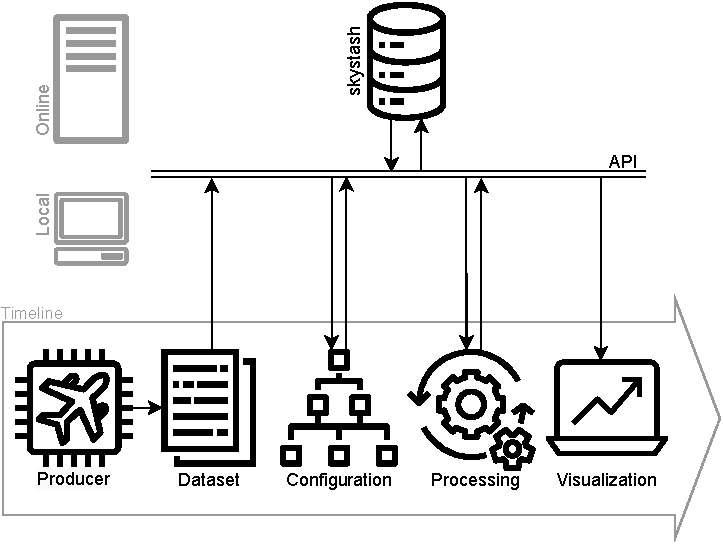
\includegraphics[width=.8\textwidth]{FT_microservices_AWS}
    \caption{The data toolchain prospectively used for Sensor Health Monitoring}
    \label{fig:fti_microservices}
\end{figure}


\section{Data Parsing}
%Since the SHM has to run on something, the original data is briefly mentioned for completeness.

Since the data the SHM will work on originates from the airplane and needs to uploaded without any modification to preserve originality this small section will deal with the handling of data from the aircraft until it reaches its destination in the skystash.

The Data is uploaded to the stash from the aircraft DAQ format. Its data is available in the proprietary IMC .raw formats. These are then parsed into the stash by converting them into timeseries for each parameter. The data structure used in the skystash is represented in figure \ref{fig:skystash_folder_structure}. The folder structure's main path is the project folder which represents the project in which the flight was performed in and contains all the project's flights. Each flight then contains parameter measurements which represent the lowest level of objects in the architecture. All objects of project, flight or measurement type can also contain JSON-usertags as well as additional data in binary format such as pdf files.

\begin{figure}
    \centering
    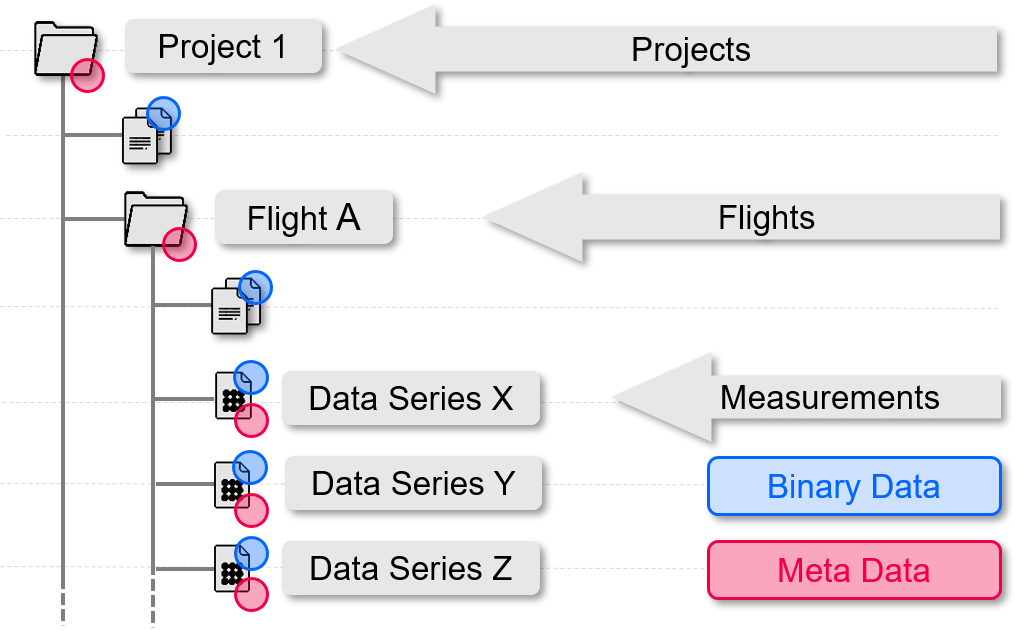
\includegraphics[width=0.5\textwidth]{skystash_folder_structure}
    \caption{skystash folder structure}
    \label{fig:skystash_folder_structure}
\end{figure}

\subsection{Parsing of ISTAR Data}
%ISTAR data originates from the ISTAR's DAQ system in the shape of .raw files for each parameter and is parsed and uploaded to the stash. It is then accessible via the stash api and can also be inspected in the stash webview. After the Dataset generation step the metadata available is only the one from the ISTAR DAQ system.
%The data is present in the shape of Projects->Collections->Series


To provide a full overview of the entire pipeline this step is mentioned. Starting off, we are left with a directory full of .raw and .imcexp files after a flight. Both are proprietary IMC formats. However, we can distinguish between both insofar that .raw files contain timeseries in an encoded format. The imcexp files then contain the configuration settings for the specific flight/measurement.

The entire directory then gets parsed by a python script. Segmenting the binary structure of the raw files and extracting the timeseries for each parameter. The DAQ and aircraft sensor config for each flight gets exported from the imcexp file and uploaded to the skystash without modification to preserve genuineness of the data as shown in figure \ref{fig:skystash_data_pipeline}. Any Metadata in shape of a JSON format is represented with a red dot and any binary formats such as pdf files or other custom data are represented with a blue dot.

\begin{figure}
    \centering
    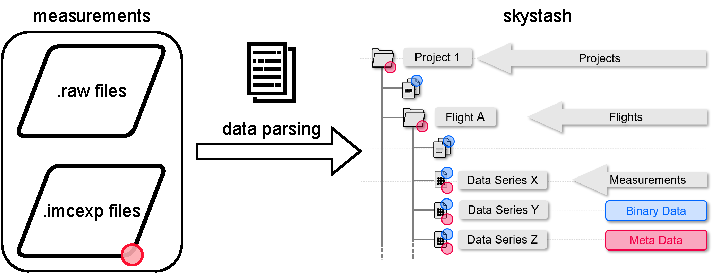
\includegraphics[width=0.8\textwidth]{skystash_data_pipeline}
    \caption{Pipeline of parsing and uploading the skystash data to the skystash without modification}
    \label{fig:skystash_data_pipeline}
\end{figure}

Parameters are saved under the flight object. Config data is assigned to the user tags of each parameter. The data is then parsed for each flight and inherent sensor.

The metadata is currently only the one from the ISTAR DAQ system. Since this metadata needs further information to make it understandable it will be enriched further within the Configuration step (See figure \ref{fig:fti_microservices}).

\newpage


\section{Configuration-Metadata}

The configuration from the previous step has now been uploaded to the skystash. It describes the actual flight-dependent DAQ configuration and changes for every flight. It is, however, not complete. Since the DAQ only saves data relevant to itself, other vital metadata for users as well as the SHM are not present. In this section a method is implemented to enrich the DAQ metadata by transforming it into a common metadata format as well as appending useful additional metadata to each sensor and the flight.

%-This step details the considerations and implementations taken to be able to generate a useful metadata model that applies necessary information to the dataset within the skystash.

\subsection{Why?}

%§ Metadata from DAQ sensible and up-to-date but incomplete
%-incomplete metadata
%-Metadata is not complete yet. -does only contain info from DAQ which represents only the info the DAQ needs. What about all the other information that is not in the DAQ?

The DAQ configuration in itself is very essential but also incomplete in that is does not yet contain necessary information for detecting errors within our data. To achieve this, we need to enhance our metadata from the DAQ with additional data. This permanent, generally unchanging metadata is first specified locally and contains values such as boundaries for level 2 or tags for level 3 to correlate parameters to each other. It is also specified for each parameter individually. It is then also possible to assign values such as frequency locally.


%§ SHM-info not available in DAQ-metadata, e.g. positional of sensors not available -shm info necessary

This necessitates a merging/fusion step of DAQ-config with the locally defined permanent metadata. This is especially useful since this locally defined metadata is not up-to-date and DAQ metada is not complete. It also Necessary to additionally add data relevant to the checks for each parameter.

%§ Input needed for SHM with all necessary infos

\subsubsection{Requirements}
%What is the Goal?

%§ Enrichment of Metadata
Leveraging these requirements we can define two goals for the configuration step.
\begin{enumerate}
    \item Enrichment of Metadata
    \item Conversion into a standardized format
\end{enumerate}
These two steps guarantee a similarity across processes which will also pay off once the SHM process may expand to other applications. The standardized format also supports the desire for FAIR principles since it allows to input data from various sources into the SHM data processing algorithm.

Additional attributes that are needed are aircraft specific information such as position of sensors within the aircraft Coordinate System (COS), the actual position of the COS relative to the aircraft and its orientation as well. For the SHM Level 2 physical limits as well as amplitudes for STFT are needed. For Level 3, only the parameter tag, defining its meaning in the application context such as \textit{static pressure} and an eventual reference parameter is defined. The reference defines context or calibration and defines the \textit{reference pressure} in the case of the \textit{static pressure}.

Generally, metadata exists in two forms. the actual flight-dependent DAQ config and the permanently valid metadata config that principally does not change. The actual config is different for each flight since it represents changes made by Flight Test Engineers to fit the DAQ-configuration the specific flight experiment. The permanent config however represents all additional info that may be relevant to a varied pool of users.


%§ Conversion into a standardized DAQ-independent format
Once a merged data construct is reached it needs to be converted into a usable, standardized format. For this step, some candidates from Internet of Things (IoT) applications have already been examined in \textcite{bodenbenner_model-driven_2022}. For the pipeline to the data processing the metadata can then be transformed into the SensOr Interfacing Language (SOIL), allowing a concise, specified format for this essential metadata.

\begin{figure}
    \centering
    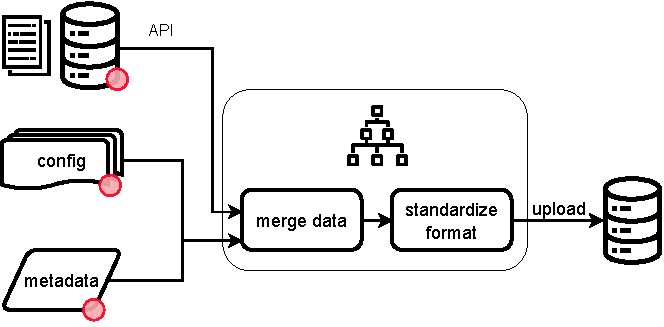
\includegraphics[width=0.7\textwidth]{skystash_metadata_pipeline}
    \caption{Metadata Pipeline}
    \label{fig:skystash_metadata_pipeline}
\end{figure}

\subsubsection{Implementation}
%implementation
%\\§ Accumulation of required metadata that needs to be supplemented
Required data then needs to be defined locally. For this, an already existing database is taken as a starting point. This database is in the shape of an excel file and will be used for development. In further steps it might be reasonable to migrate this database to a different format to guarantee true provenance for configuration information. However, this is reserved for a later point. It suffices for now and will be expanded for columns that can add attributes for each parameter such as the aforementioned level 2 and 3 requirements and also additional data that may be of interest for users in the skystash such as sensor position in the aircraft. This is shown in figure \ref{fig:skystash_data_pipeline} within the config and metadata elements that represent permanent config info and the metadata for the steps.

The metadata fusion is part of the feedback loop that is in-line with the data processing and feedback. So this step is essential to the process since previously all steps from the SHM-toolchain figure \ref{fig:fti_microservices} had to be performed previously if there had been any marginal changes. Compartmentalizing and modularizing these single steps allows to then accelerate development and testing by not having to parse data within each iteration.

%-The configuration of the ISTAR is of great importance for the data processing. Also of great importance is the knowledge database which is currently in the shape of an excel document.
Also, attributes that are generally transmitted within the DAQ configuration are sampling rates, data origins and other miscellaneous information related to the system. Not contained are information about general sensor description, position of sensors, overall setup of the aircraft sensor architecture and check limits for data values. To preserve the original DAQ infos as closely as possible the merging step as portrayed in figure \ref{fig:skystash_metadata_merging} is proposed. This way, original DAQ info that is frequently changing such as the frequency gets preserved while still allowing additional data by the permanent local config to be used

%\\§ Fusioning of Metadata with Priorization of DAQ data
The metadata enrichment process is described in Figure \ref{fig:skystash_metadata_pipeline} starting with data and metadata that is available in the skystash and unmodified. This unmodified data then gets enriched with metadata for parameters that are not already described by the DAQ config. In this step other SHM attributes get assigned such as checking limits for level 2 and variable tags for level 3 defining the meaning of a parameter. Since the metadata uploaded to the stash in itself is not very expressive and cryptic it needs to be refined further into a usable, concise format.
\begin{figure}
    \centering
    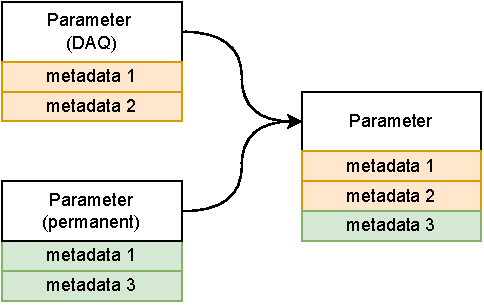
\includegraphics{skystash_metadata_merging}
    \caption{Priority Merging of Skystash data. Using the actual-DAQ configuration to overwrite other metadata.}
    \label{fig:skystash_metadata_merging}
\end{figure}


%\\§ Then translation/conversion into standardized SOIL format
As previously discussed in chapter \ref{chap:2-metadata-format}, a common format for exchanging metadata is needed. Following Fusion, the data is now available in a JSON format that contains the previously defined attributes for each parameter. To increase standardization a further conversion into the SensOr Interfacing Language is considered. This could increase acceptance and standardization since it is starting to be increasingly used within IoT contexts. A proposed structure would contain single sensors as parent elements and components containing the appended attributes. \cite{behrens_domain-specific_2021}

\subsubsection{Summary}
%§ Generating additional metadata
A central format for metadata has now been agreed upon. Especially data flows have been determined which strongly facilitates further development by structuring input and output operations. Primarily, the place to define further metadata attributes has been defined and the step to compile it within the configuration data merge step. Naturally, this will have to be changed further within further development. This method however condenses work into one single place.
%§ Fusion of metadata sets
The incomplete metadata from the DAQ has been enriched with the locally available metadata such as additional knowledge about the aircraft, the sensors itself and its context. Also, necessary data for the SHM step has been added such as limits for checks as well as tagging parameters for physical correlation checks which has been fused into a single data structure.
%§Conversion into standardized format
After compiling various inputs into a single metadata structure a common format has also been found. SOIL has been examined for usage and implementation is intended for future use.

\newpage


\section{Data Processing}
Now, we can sort out the vital step of this work. Taking the inputs of data and metadata with the configuration needed and implementing sensible logic to reliably detect anomalies in the data. This will first be preceded by some considerations about software architecture and then delving into the specific methods for FMEA.

\subsection{Software architecture considerations}
%todo: check mention of :				□ Modularity	□ Modifiability □ Reusability □ Quick Feedback


Careful consideration needs to be given to the workflow of the level 1 check to allow scalability and reduce manual interaction. To achieve this architecture manual steps are reduced as far as possible. However, some level of configuration must be implemented otherwise only relational sensor behavior could be detected. Meaning that sensor faults occurring temporarily within an experiment can be detected but permanent behavior is not noticed by a relative algorithm e.g. only detecting strong aberration. To satisfy this desire for information the preceding metadata configuration step in chapter \ref{chap:2-metadata-format} is implemented.

\subsection{Check 1 Implementation}
For implementing the level 1 checks, the measured data needs to be compared to the expected data. To gain insight into what the expected data is, the configuration file of the data acquisitioning system needs to get parsed as presented in chapter \ref{chap:2-metadata-format}.

It is possible to export the DAQ flight-specific configuration within the software \textit{IMC Studio}. This reads .imcexp files and then allows export into a .xml format. Downsides are though that various manual steps are involved in this process and it is thus prone to errors. So, we naturally attempt to automate it.

It turns out that the DAQ's imcexp format is in fact a .zip directory. The 7zip command line tool allows opening the configuration file since the configuration file's format is not fully complying to the zip standard making several python libraries fail during the process. This stems from an issue with the zip header and footer parts of the file that are not at expected places (effectively in the front and back). Once opened, the configuration file contains multiple files as well as an essential xml file that contains the needed sensor metadata. After some formatting these .imcexp can be read straight to generate similar info to the \textit{IMC Studio} workflow.

The expected data then can be extracted from the .imcexp files and allows quick comparison against the actually generated data. This resolves the Level 1 implementation.

\subsection{Check 2 Implementation}

Within Level 2, the sensor timeseries get checked by themselves without contextualization of other sensor data. This gets accomplished by principally checking them against predefined limits as shown in figure \ref{fig:level_2_flow}.

Use Cases for this are primarily the two implementations:

\begin{enumerate}
    \item unmodified signal
    \item noise amplitude by using STFT amplitude \ref{chap:2-plausibility}
\end{enumerate}

\subsubsection{Methods}

The general workflow consists of getting the timeseries of the signal from the skystash database, then transforming it in some respect and then checking it against limits.
%how it works
%• How does it generally work?
%□ It checks all parameters against a range and notes the values and timestamps where limits where exceeded.
%□ It then saves them into a json file for the type of check that was performed (value out of limits, movement out of limits

\begin{figure}
    \centering
    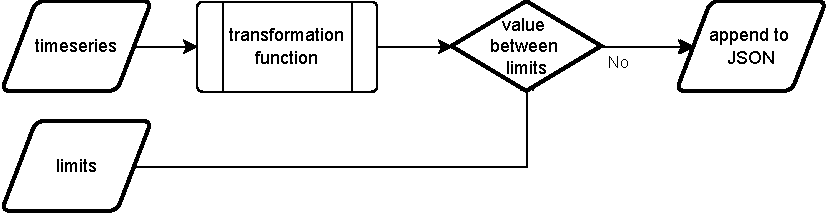
\includegraphics{level_2_flow}
    \caption{Checking Logic for every type of level 2 function.}
    \label{fig:level_2_flow}
\end{figure}

The logic in this step can then generally be summarized in equation \ref{eq:level_2} with $l$ being the limit that is checked against.
\begin{equation}
    f_{report}(t) = \left\{\begin{array}{rcll}
                               t:True & \mbox{for} & f_{value}(t) < l_{min} \vee f_{value}(t) > l_{max} \\
                               None   & \mbox{for} & l_{min} < f_{value}(t) < l_{max}
    \end{array}\right
    \label{eq:level_2}
\end{equation}

The context $f_{value}(t) = g(f(t))$ is additionally used. Representing any transformation operation as the function $g$.

\subsubsection{Invalid value}

A check implementation counterchecking the sensors sampling that generates fault detections based on deviation from predefined sampling. This takes into account the DAQ config since it contains the current sampling rate. Minimizing false positives.

This method is necessitated by the simple absence of \textit{None} or any kind of invalid values in the skystash. Meaning that such values are simply not present. To detect \textit{None} values we then are presented with two options:

\begin{enumerate}
    \item check parameter start and stop time
    \item check sampling rate
\end{enumerate}

We could also check for values remaining unchanged for longer times. This will be part of the section of \textit{sensor movement} mentioned below.

\subsubsection{Out of range}
Generally, predefined limits are checked within SHM Level 2. For the first step, values are checked whether they are within a predefined range. This means ranges such as defined in Table \ref{tab:level_2_range}. Of course, this selection is biased and may not be accurate for most mission profiles like atmospheric research aircraft that cruise in altitudes of up to 45,000 ft MSL.

% Please add the following required packages to your document preamble:
% \usepackage{booktabs}
\begin{table}[]
    \centering
    \begin{tabular}{@{}lll@{}}
        \toprule
        Parameter           & Minimum & Maximum   \\ \midrule
        Barometric Altitude & -1000ft & 40,000ft  \\
        Static Pressure     & 1Pa     & 120,000Pa \\ \bottomrule
    \end{tabular}
    \caption{Exemplary limits for checking parameters}
    \label{tab:level_2_range}
\end{table}

\subsubsection{Movement check}
\label{chap:4-level_2_movement}
The next category examining the sensor behavior can be classified into sensor movement being too low or sensor movement being too high. Movement being defined within this context as the difference of a new sensor value to the previous one.

Hence, an approach using a STFT is chosen in which the amplitude is averaged across all frequencies from its spectrum. This guarantees a generalized feature extraction, resulting in standardization for parameters. Based on this spectral analysis, the logarithmic order of the variable can be estimated within its dataset. Previously, the frequency is assumed via time difference of start and end time divided by $n_{datapoints}$. The STFT also implements preprocessing steps that would otherwise be necessary such as translating the signal by its average value as well as scaling it by its standard deviation. Would one be interested in examining a signal using functions from a statistical toolbox, a similar result may be achieved by performing the previous steps of averaging and scaling the signal and then examining the variance within a moving window of the signal, similar to the STFT. The size of the moving window for such an analysis is defaulted to 256 data points for each signal. Certain issues with methods of moving windows are however, that they are not very meaningful for the beginning and ending of datasets within which the window is not fully occupied. This may lead to spikes for the STFT, which is why it is found that the STFT is generally more powerful to examine insufficient sensor movement.

This can be described in equation \ref{eq:level_2_movement_check} as:
\begin{equation}
    g(f(t)) = \frac{1}{n}\sum_{m}^{n} F(m,t)
    \label{eq:level_2_movement_check}
\end{equation}
\begin{conditions}
    m                          & frequency                                 \\
    n                          & amount of frequency points                \\
    X(m,t) = \mbox{STFT}(f(t)) & the STFT of f \cite{smith_scientist_1999} \\
\end{conditions}

\newpage

\subsection{Check 3 Implementation: }


Aims of Level 3 Implementation are to model the aircraft's state in a reference system. Parameters are present in various reference systems as well as in redundancy. Within this section the issues arising from the merging from parameters will be the main topic, accompanied by how to implement the necessary data.

First, a common reference state will be defined for checks, then the Parity function \cite{chap:parity_equation} will be implemented and then the topic of how to deal with data input and output on a large scale will be discussed.

\paragraph{Finding a reference state}

%And
As discussed, many parameters are available that allow backtracking onto a single state variable of the aircraft. They are also available in various COS.

%But
Aircraft position and state can be interpreted in various Coordinate Systems. It is also necessary to compare redundant parameters within these varied reference systems. Hence, the reduction of the various reference systems onto a single reference system is necessary to guarantee comparability.

%Therefore
Since the geodetic reference system is best described by the GNSS and Inertial Measuring Unit (IMU) it will be used in the following as a reference system for calculations. Additionally, moving aircraft coordinate systems like the aerodynamic and the along track Coordinate system may be derived using known transformation angles and velocities. \cite{brockhaus_flugregelung_2011}


%Interfacing: Clean interfaces are generated throughout the model. Enabling a standardized state vector x. Meaning that A remains standardized for any aircraft while B, U and L need to be adjusted for any changes to the aircraft or sensor data.
%A starting point which shall be considered is the geodetic reference. it measures the aircraft's position by its displacement from the previously (ref?) discussed WGS84 system. Meaning that altitude gets measured as the orthometric height (see ellipsoid height-geoid height).
%Latitude and Longitude form the x and y axis of the COS. True heading forms the reference heading within the geodetic system.
%All aircraft parameters related to motion and position of the aircraft should be attempted to be condensed into this form.

%The integration step may be omitted in early design stages since the necessary equations and equilibriums of Forces and Moments could only be modelled linearly while neglecting various unknown factors like shifting CG due to fuel burn, actual Inertia of Aircraft and aircraft mass. Hence, this step may be implemented if time allows it.

\paragraph{Dynamic configuration and correlation of parameters}

The necessary configuration for the Parity Equations should then be expandable and dynamically adaptable. This means creating a dynamic structure that allows to represent the complex physical aircraft correlations. This includes creating hierarchical configuration information and an algorithm that reads this configuration and then downloads the sensors from the skystash to include them into the essential Level 3 flow represented in figure \ref{fig:level_3_flow}. The detected anomalies then get uploaded to the skystash.

\begin{figure}
    \centering
    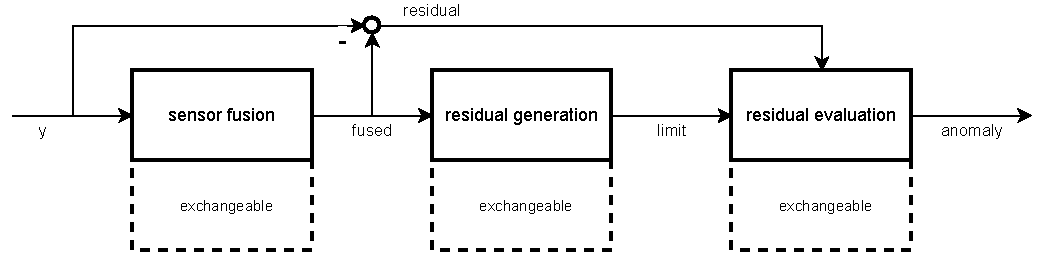
\includegraphics[width=0.8\textwidth]{level_3_flow}
    \caption{Vector of $y$ is merged in a sensor fusion step to then generate a residual. Limits to evaluate the residual are then generated in the next step followed by the residual evaluation determining if the value is anomalous.}
    \label{fig:level_3_flow}
\end{figure}

For the Level 3 configuration and information assignment a data structure similar to the SensOr Interfacing Language is proposed. An exemplary structure is shown in figure \ref{fig:level_3_config}.
\begin{figure}
    \centering
    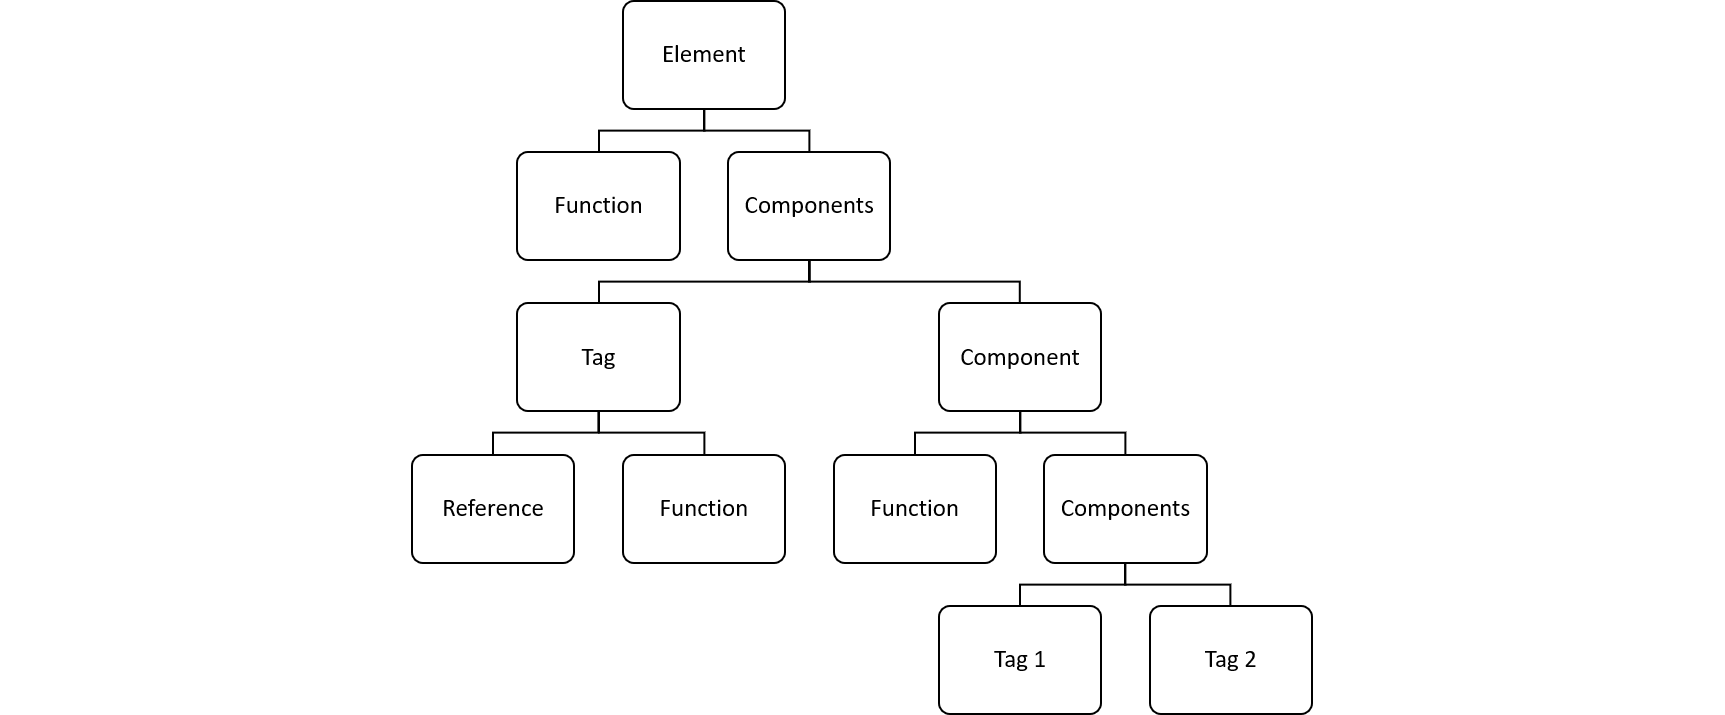
\includegraphics[width=\textwidth]{level_3_config}
    \caption{General structure of physical correlation setup}
    \label{fig:level_3_config}
\end{figure}

This dynamic description for parameter correlations is required in order to implement an efficient and quick way to assign parameter correlations. It is then assumed that a tree structure is fit for this task since parameters can be correlated to other upstream parameters by using a single flow direction. A more detailed view in a Universal Markup Language (UML) graph is shown in figure \ref{fig:level_3_config_uml}. The Class component generally forms the common element in the structure as seen in figure \ref{fig:level_3_config}. It is also notable that Tags as well as Elements inherit from the Components Class and are instances of it. Components possess the attributes of other \textit{components}, their own \textit{name}, the \textit{merged parameter} which represents a single fused value for all parameters below and an attribute containing all lower lying parameters called \textit{all parameters} which contains all parameters. It also contains two functions for firstly merging its components into the merged value and secondly transforming its parameters into a desired state dimension. E.g. converting Static Pressure into a barometric altitude. The current default of these functions consists of relatively rudimentary logic to not transform the parameter and to take the average of values to merge various parameters.

The inheriting entity \textit{Tag} mainly differs from the \textit{Component} in that it does not contain any subcomponents and contacts the skystash to gather all variables from the database containing the tags that are represented by its name. An optional attribute is a reference or calibration value that is assigned in the permanent configuration database (See chapter: \ref{chap:2-metadata-format}).
%reference to DAQ and "permanent" database.
The entity \textit{Element} represents the parent node of the configuration tree. Its only difference to a regular \textit{Component} is that it allows to keep multiple merged_parameters in its view to e.g. allow altitude and speed to coexist and not get erroneously merged.

\begin{figure}
    \centering
    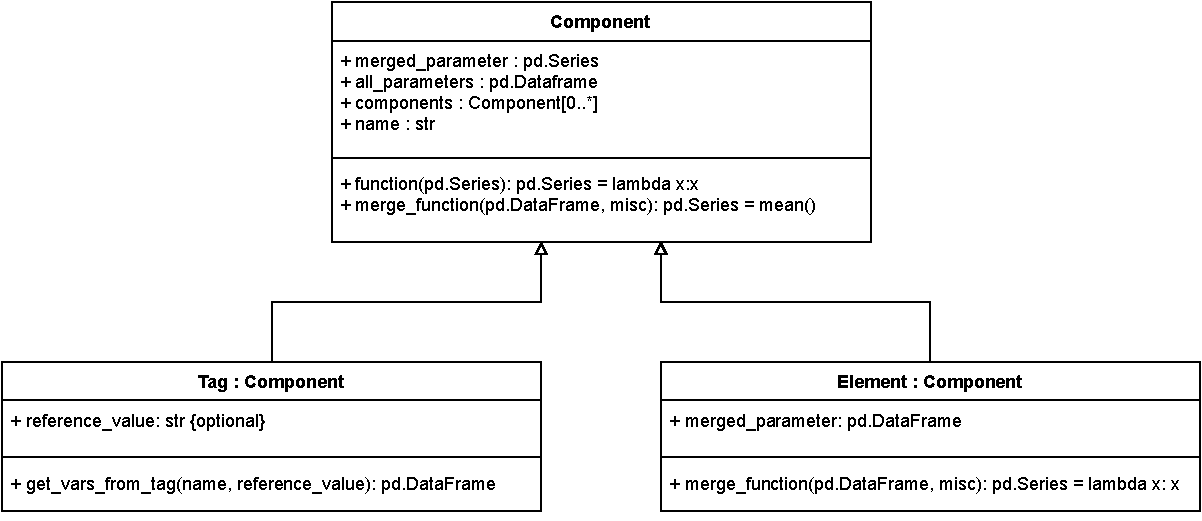
\includegraphics[width=\textwidth]{level_3_config_uml}
    \caption{Description of the Level 3 JSON check configuration}
    \label{fig:level_3_config_uml}
\end{figure}

%□ Parity implementation within hierarchical method
Using this configuration method, the Parity model can then be calculated using given methods to transform and fuse the data. This starts by parsing the configuration structure, downloading sensors for each Tag and fusing sensors y into a fused value as defined in the configuration and as shown in figure \ref{fig:level_3_flow}.
%□ Flow structure
%□ Config file explanation


%In figure \ref{fig:level_3_config, fig:level_3_config_uml} the general structure of the dynamic configuration in JSON format is shown. The configuration parent is a component containing subcomponents that themselves may contain subcomponents.

This system takes inspiration and inherits the configuration structure from the SensOr Interfacing Language (SOIL)\cite{behrens_domain-specific_2021}. In this work's use-case the \textit{Element} ISTAR research aircraft contains top-level components that are the independent state variables of the aircraft. An example that will be invested further in following sections is that of the \textit{static pressure}. The workflow begins by defining the Tag \textit{static pressure} in the permanent configuration and then configuring it into the Level 3-configuration structure. This tree structure is then parsed and calculates a value for each level of detail taking into account its lower lying neighbors. Some weighting also has to be considered since a number of redundant pressure sensor could skew results against a single GNSS parameter. Thus, a condensed parameter is calculated for each degree of freedom that is based on predefined algorithms and tags that can be freely defined within the config file that are then recursively parsed within the tree structure.
%avoid weighting by structuring checks into a tree format for independent aircraft state variables.

\paragraph{Limit Generation}
Now the fused state value as well as the single, transformed sensor values are present. The next step consists of defining a limit for the resulting residual from combining the fused state with the single sensor value. Naturally, this could be defined manually by e.g. defining a limit of 0.5 meters for an altitude value. Since however automation is sought after, an automatic limit generation is determined as a requirement for dealing with these large data sets.

Statistical methods then are examined for automatically generating thresholds for the parameter values. A method is then implemented to detrend the signal and take the resulting noise as the allowed deviation. In practice this results in a rudimentary high-pass filter (HPF) that gets realized by using a moving window function combined with an averaging function with a window width of $n=256$. After using this crude HPF to extract noise from the dataset we can acquire the standard deviation of this noisy signal and use it to set the limit for resulting residual evaluation.

%TODO: plot here to visualize action

\paragraph{Residual Interpretation}

After generating the residual as well as the limits for the checks anomalous values get detected by checking whether they are outside the allowed range (see equation \ref{eq:level_2}).

Using this generic approach primarily guarantees quick and easy operations. It remains yet to be seen, how well other methods might perform compared to it. A manually defined residual limit then might guarantee more custom boundaries and using a probability density function (PDF) implemented in works such as \cite{svard_data-driven_2014} may also promise to deliver good results but nonetheless exceeds the scope of this work.

%Based upon the previously defined hierarchical model for Parity Equations residuals are generated based upon the difference of the parameters to the top level parameters (Single, fused value) and the single transformed sensor values (All Parameters) as previously discussed in Table \ref{tab:states_and_signals}.


\newpage


\section{Report Visualization}

At this point, the data has been checked and a report within a JSON-format has been generated and appended to the skystash flight. The missing parameters have been found, sensor values have been checked by themselves and additionally physical correlations and redundant sensors have been checked. However, FMEA algorithms generally need some tuning to become their most effective and analyzing the JSON data takes some time to grasp all peculiarities of the data. Facilitating and Accelerating development, the STASHBOARD is introduced. It is an interactive data report that is developed for data analytics. And instead of a pdf type report it works more efficiently and rather follows the paradigm of a single source of truth. It allows for dynamic updates and thus does not represent a data source in itself but rather view on the source facilitating updates on the data. It allows to quickly gain an overview over the state of sensors and closes the feedback loop in the development cycle.

\subsection{Visualization}
\label{chap:4-visualization}
A main paradigm of this visualization is that it prioritizes qualitative over quantitative design. Meaning that it does not mention explicit details but allows to comprehend and retrace the qualitative FMEA results. It shall be a UX-centric design with the possibility of identifying outliers or oversensitive SHM config parameters. With Level 1 of the SHM giving a quick overview over Sensor Availability and Level 2 serving as a simple check for any anomalies. Level 3 then serves as a more meaningful way to identify problems in the datasets by showing parameter relations and identifying deeper lying faults.

\paragraph{Timeline}

Often, sensors may deliver erroneous or faulty values which get discarded along the workflow. These values are then plainly missing from the dataset. The Timeline attempts to solve this problem by generating a central overview over start and stop times of each sensor's measurement period. Complementing the timeline with the sampling rate check in Level 2 serves as a method to reliably detect missing sensor values. The Timeline's implementation is shown in figure \ref{fig:stashboard_timeline}.

\begin{figure}[!h]
    \centering
    \begin{subfigure}[b]{1\textwidth}
        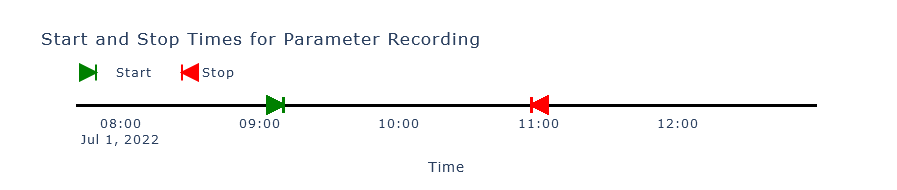
\includegraphics[width=0.8\textwidth]{stashboard_timeline}
        \caption{The sensor timeline}
        \label{fig:stashboard_timeline_clean}
    \end{subfigure}
    \begin{subfigure}[b]{1\textwidth}
        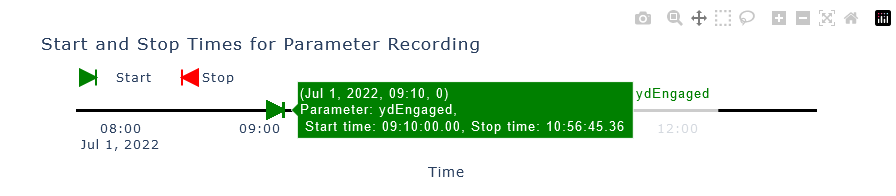
\includegraphics[width=0.8\textwidth]{stashboard_timeline_interactive}
        \caption{Interactive tooltip when hovering over a marker}
        \label{fig:stashboard_timeline_interactive}
    \end{subfigure}
    \caption{The Sensor Timeline allows insights into the measurement periods of sensors}
    \label{fig:stashboard_timeline}
\end{figure}

The sensor primarily delivers a clean view showing markers for each sensor measurement with start markers being green and stop markers being red in figure \ref{fig:stashboard_timeline_clean}. Once additional information is desired related to an outlying sensor measurement the tooltip of a marker (see figure \ref{fig:stashboard_timeline_interactive}) shows parameter Name as well as the parameter's precise Start and Stop Time. Allowing further investigation by using the skystash architecture.

\paragraph{Parameter Availability}
After monitoring, a list of missing parameters is generated. To show and detect this info quickly, a speed gauge style display is chosen to display this scalar value as shown in figure \ref{fig:stashboard_speedo}.

\begin{figure}[!h]
    \centering
    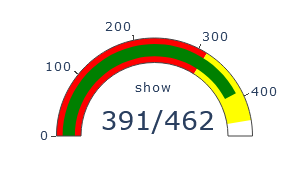
\includegraphics[width=0.4\textwidth]{stashboard_speedo}
    \caption{Displaying the available number of parameters}
    \label{fig:stashboard_speedo}
\end{figure}
The red value is representing the percentage of the standard deviation ($\sigma=68.27\%$) and the yellow area represents double the standard deviation ($2\sigma=95.45\%$).

\paragraph{Level 2: Singular Sensor Examination}
To quickly get an overview of missing parameters a method to show cumulative errors over the flight is developed (see figure \ref{fig:stashboard_level2}).

\begin{figure}[!h]
    \centering
    \begin{subfigure}[b]{1\textwidth}
        \centering
        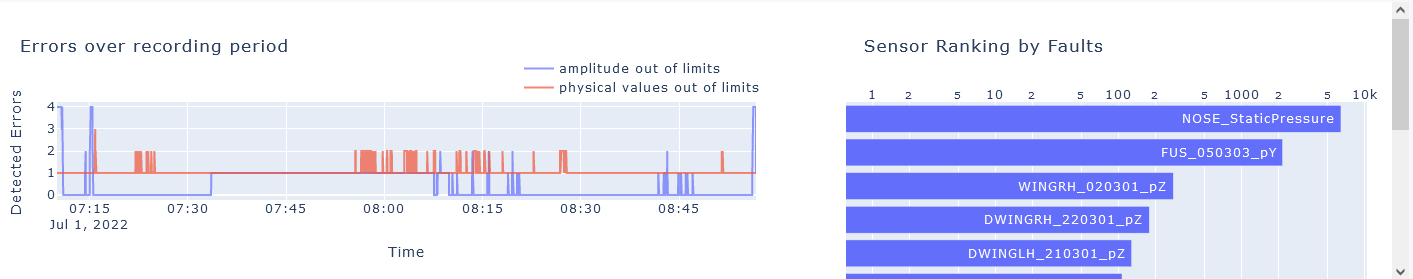
\includegraphics[width=\textwidth]{stashboard_level2}
        \caption{Detected cumulative Faults over time (left), sensors ranked by number of faults (right)}
        \label{fig:stashboard_level2_clean}
    \end{subfigure}
    \begin{subfigure}[b]{1\textwidth}
        \centering
        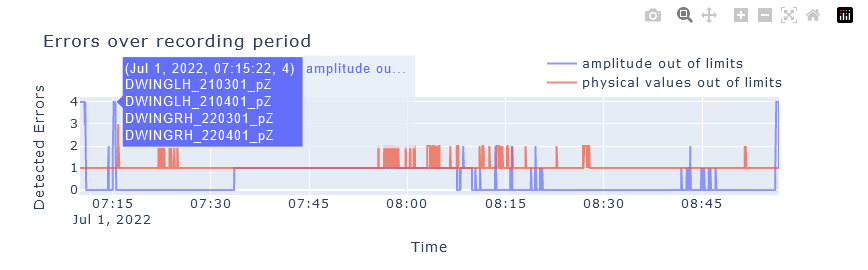
\includegraphics[width=0.9\textwidth]{stashboard_level2_interactive}
        \caption{Interactive tooltip showing anomalous sensors at timestep}
        \label{fig:stashboard_level2_interactive}
    \end{subfigure}
    \caption{Single Sensor Analysis shows cumulated faults over measuring period and a sensor fault ranking}
    \label{fig:stashboard_level2}
\end{figure}

For each type of fault cumulative errors at a given timestep are added across sensors. Then the total number of errors is compounded for each sensor and displayed in a graph bar ranking.
Specific points of interest on the graph can closer be examined by hovering over them as shown in figure \ref{fig:stashboard_level2_interactive}. The tooltip then shows the exact time of anomaly as well as the detected errors.


\paragraph{Level 3: Examining Sensor Interactions}

The Sensor Interaction and correlation is calculated for each sensor. To then grasp the checked correlations a tree map is employed to display the hierarchical relations that is provided by the SHM-Level 3 configuration file (left in figure \ref{fig:stashboard_level3}).

\begin{figure}
    \centering
    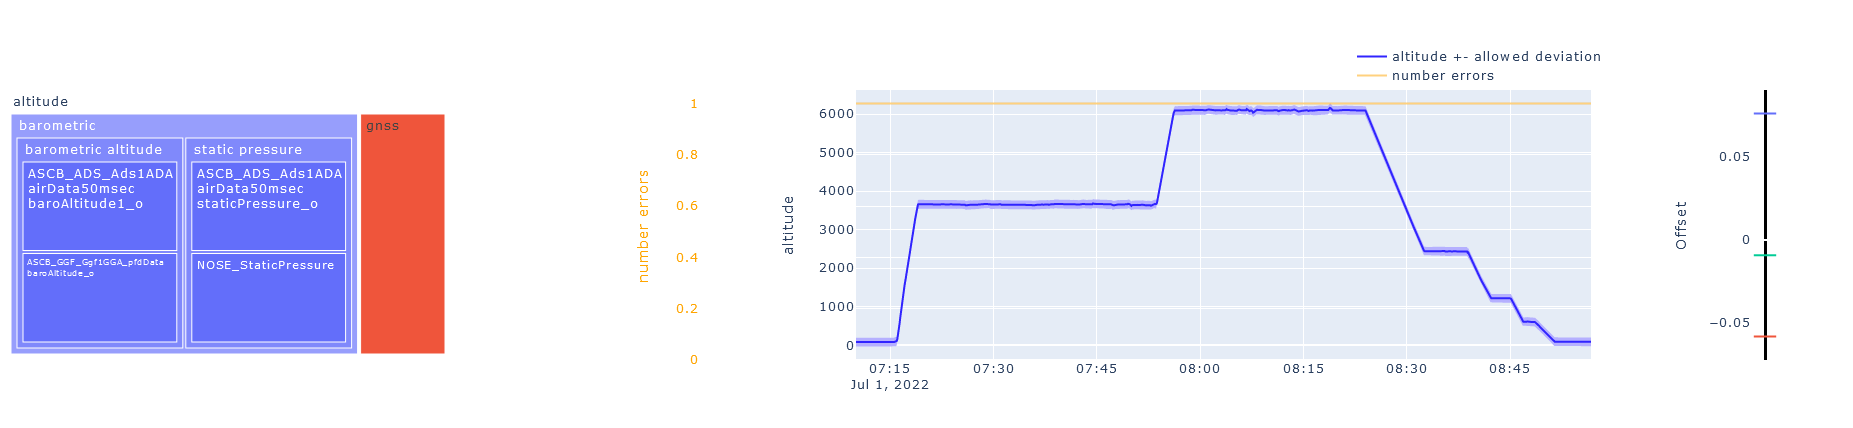
\includegraphics[width=\textwidth]{stashboard_level3}
    \caption{Level 3}
    \label{fig:stashboard_level3}
\end{figure}

Then, the fused state value associated with its upper and lower limits is displayed in the following window. Overlaid, the amount of detected sensor errors is shown, similar to figure \ref{fig:stashboard_level2_clean}. Finally, the average of the residual for each parameter is shown to quantify any occurring bias in the right window.


\paragraph{Implementation}
To feed these displays a data pipeline is needed. The generated JSON-report file can be used to fulfill this job by feeding the flight SHM data to the Timeline, Level 1 and Level 2. For Level 3 the parameter SHM-metadata is needed as shown in figure \ref{fig:stashboard_flow}.

\begin{figure}[!h]
    \centering
    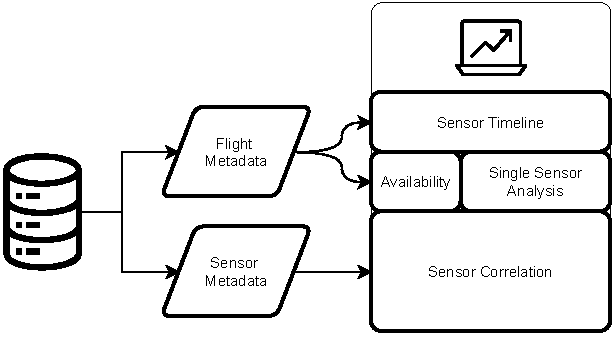
\includegraphics[width=0.8\textwidth]{stashboard_flow}
    \caption{Data Pipeline for Stashboard elements to display SHM reports}
    \label{fig:stashboard_flow}
\end{figure}

The flow of the Stashboard allows selection of any stash flight by using the skystash API through dropdown menus. The Stashboard can then access the flight's metadata and represent it by using the previously developed data displays.
%\begin{figure}
 %   \centering
  %  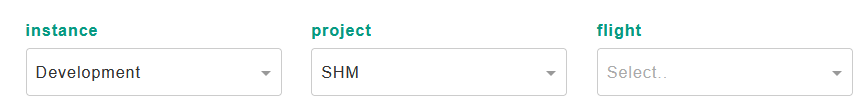
\includegraphics[width=\textwidth]{stashboard_flight_selection}
   % \caption{Selecting any flight using dropdown menus}
   % \label{fig:stashboard_selection}
%\end{figure}
This results in a flexible, scalable analytics application for skystash data and SHM reports that gives a quick overview over the vast amounts of data and be used by flight test engineers to get an overview over data quality as well as developers to optimize algorithms. The first prototype of the developed application is shown in figure \ref{fig:stashboard}.

\begin{figure}[!h]
    \centering
    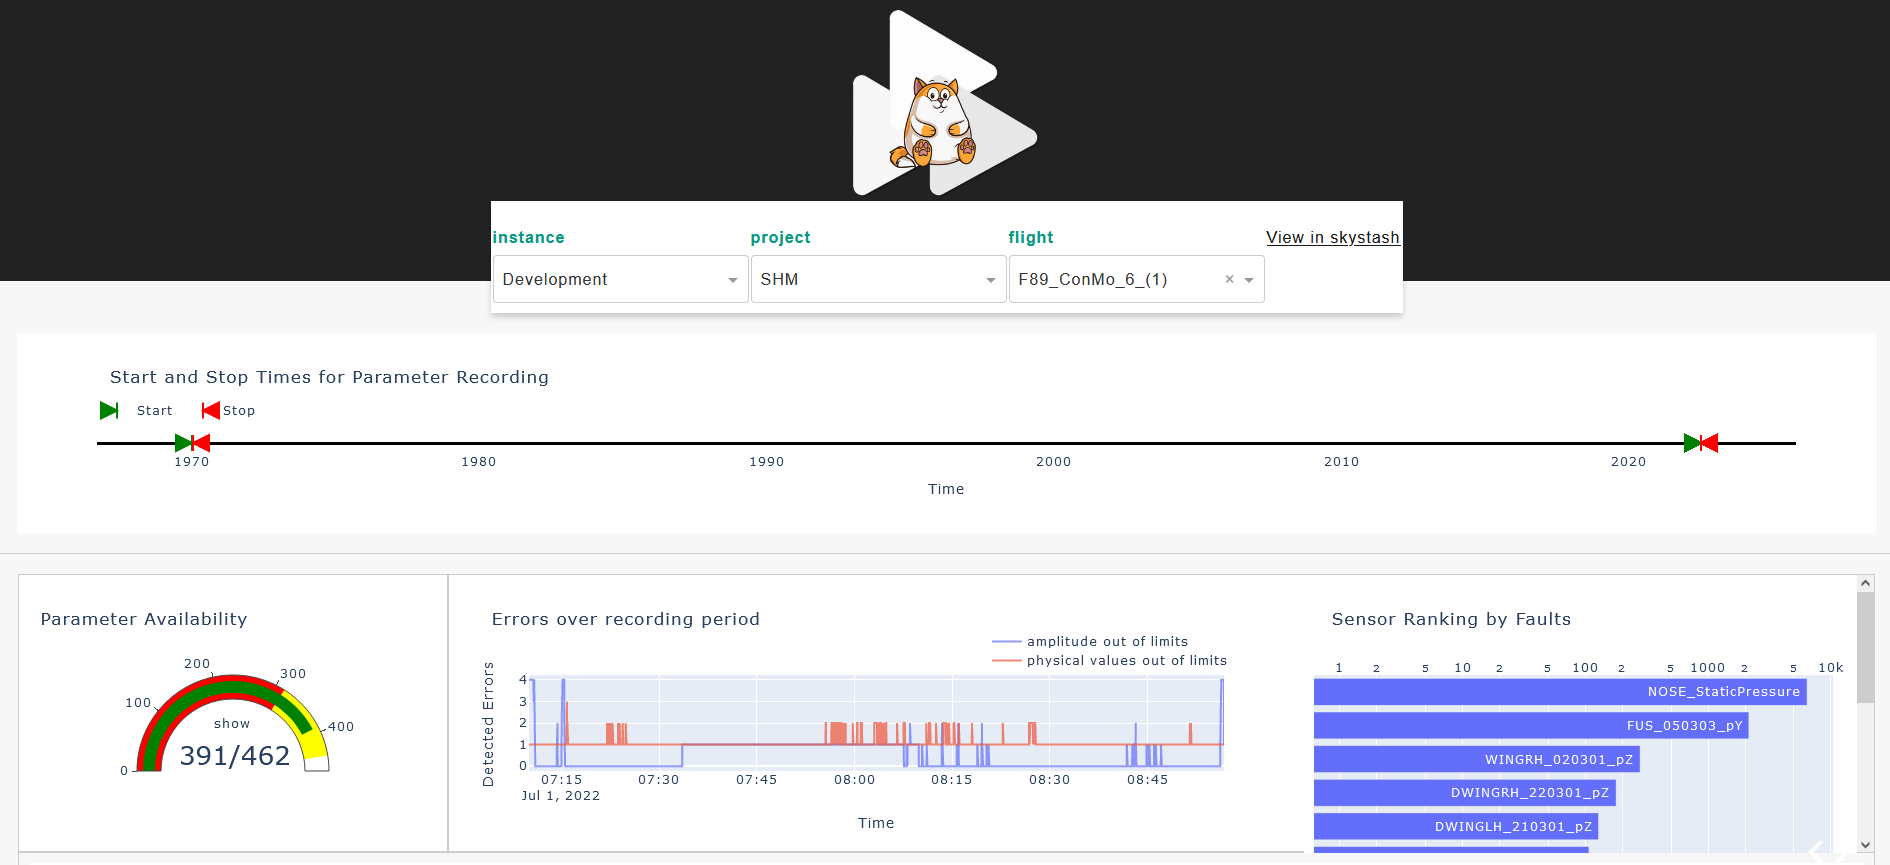
\includegraphics[width=\textwidth]{stashboard_screenshot_1}
    \caption{Stashboard webbased analytic Tool }
    \label{fig:stashboard}
\end{figure}


\newpage
\section{Summary}

This parameter showed the methods used and the considerations made for the implementation of this SHM. Various methods and approaches were implemented to check for sensor faults. Next to the straight implementation, focus was put into developing solid interfaces to ease further implementation of future methods of fault detection. This applies for Levels 1, 2 as well as 3 which in this work was only minimally implemented to allow this prototype to see the light of day.





